\section{Free groups, free products, generators and relations}
\begin{ex}
    Every nonidentity elements in a free group $F$ has a infinite order.
\end{ex}

\begin{answer}
    Define the length of a word $x=a_{1}^{\lambda_{1}}a_{2}^{\lambda_{2}}\cdots a_{n}^{\lambda_{n}}$ is $n$ and denote it as $len(x)$. Assume $len(x)=n$ for some $n\in F$ and $len(1)=0$, we prove that $len(x^{m})\geq n\forall m\geq 1$.

    Let $k$ be the largest integer such that  $a_{n-j}^{\lambda_{n-j}}=a_{n}^{-\lambda_{j}}$ for $j=0, 1, \dots, k-1$. If $k>\left[\frac{n}{2}\right]$. For even $k$, $a_{\frac{n}{2}}^{\lambda_{\frac{n}{2}}}=a_{\frac{n}{2}+1}^{-(\lambda_{\frac{n}{2}+1})}$, $a_{\frac{n}{2}-1}^{\lambda_{\frac{n}{2}-1}}=a_{\frac{n}{2}+2}^{-(\lambda_{\frac{n}{2}+2})}$, $\cdots$ which means $x=a_{1}^{\lambda_{1}}a_{2}^{\lambda_{2}}\cdots a_{n}^{\lambda_{n}}=1$. For odd $k$, $a_{\left[\frac{n}{2}\right]+1}^{\lambda_{\left[\frac{n}{2}\right]+1}}=a_{\left[\frac{n}{2}\right]+1}^{-(\lambda_{\left[\frac{n}{2}\right]+1})}$, which is contradictory to $x$ is reduced. So $k\leq \left[\frac{n}{2}\right]$.

    Divide $x=x_{1}x_{2}x_{3}$ where $x_{1}=a_{1}^{\lambda_{1}}\cdots a_{k}^{\lambda_{k}}$, $x_{2}=a_{k+1}^{\lambda_{k+1}}\cdots a_{n-k}^{\lambda_{n-k}}$, $x_{3}=a_{n-k+1}^{\lambda_{n-k+1}}\cdots a_{n}^{\lambda_{n}}$. $x_{3}x_{1}=1$. So $len(x)=len(x_{1})+len(x_{2})+len(x_{3})=n$. $x^{m}=x_{1}x_{2}x_{3}x_{1}x_{2}x_{3}\cdots x_{1}x_{2}x_{3}=x_{1}x_{2}^{m}x_{3}$. $len(x^{m})=len(x_{1})+m\cdot len(x_{2})+len(x_{3})\geq n$. So $\forall m\geq 1$, $x^{m}\neq 1$, $\left| x \right| $ is infinite.
\end{answer}

$$ $$

\begin{ex}
    Show that the free group on the set $\{a\}$ is an infinite cyclic group, and hence isomorphic to $\mathbf{Z}$.
\end{ex}

\begin{answer}
    $F(\{a\})=\left\langle a\right\rangle$ and thus it's a infinite cyclic group. $F(\{a\})\cong \mathbf{Z}$.
\end{answer}

$$ $$

\begin{ex}
    Let $F$ be a free group and let $N$ be the subgroup generated by the set $\{x^{n}|x\in F, n\text{ a fixed integer}\}$. Show that $N\lhd F$.
\end{ex}

$$ $$

\begin{ex}
    Let $F$ be the free group on the set $X$, and let $Y\subset H$. If $H$ is the smallest normal subgroup of $F$ containin $Y$, then $F /H$ is a free group.
\end{ex}

\begin{answer}
    We prove $F /N=\left\langle (x /Y)N\right\rangle$. For any $x\in F$, $x\notin N$, assume $x=x_{i_{11}}x_{i_{12}}\cdots x_{i_{1m_{1}}}y_{j_{11}}y_{j_{12}}\cdots y_{j_{1n_{1}}}x_{i_{21}}\cdots$, where $x_{i_{11}}$, $x_{i_{12}}\cdots\in X$ and $y_{j_{11}}\cdots\in Y$. Denote $x_{1}=x_{i_{11}}\cdots x_{i_{1m_{1}}}$, $x_{2}=x_{i_{21}}\cdots x_{i_{2m_{2}}}$ $\cdots$. $y_{1}=y_{j_{11}}\cdots y_{j_{1n_{1}}}$,  $y_{2}=y_{j_{21}}\cdots y_{j_{2n_{2}}}$ $\cdots$. The index should be finite. WLOG, assume the maximal index of $x_{i}$ and $y_{i}$ are the same $k$. Then $x=x_{1}y_{1}\cdots x_{k}y_{k}$, where $y_{i}\in \left\langle Y\right\rangle$ is a normal subgroup. So $x=x_{1}\cdots x_{k}y_{1}\cdots y_{k}$, $xN=x_{1}\cdots x_{k}y_{1}\cdots y_{k}N=x_{1}\cdots x_{k}N$. $xN\in \left\langle (X/Y)N\right\rangle\Rightarrow F /N\subset \left\langle (X /Y)N\right\rangle$. $\left\langle X /Y\right\rangle < F$ and $\forall a_{1},a_{2}\in \left\langle X /Y\right\rangle$, $a_{1}a_{2}^{-1}\notin N$ so $\left\langle(X /Y)N\right\rangle< F /N$. Thus $F /N=\left\langle (X /Y)N\right\rangle$.
\end{answer}

$$ $$

\begin{ex}
    The group defined by generators $a,b$ and relations $a^{8}=b^{2}a^{4}=ab^{-1}ab=e$ has order at most 16.
\end{ex}

\begin{answer}
    It's not difficult to see $a^{8}=b^{4}=e$. We only need to check $a^{i}b^{j}$ and $b^{j}a^{i}$ with $0\leq i\leq 7$ and $0\leq j\leq 3$. $ab=ba^{-1}-ba^{7}$, $b^{2}=a^{-4}=a^{4}$, so we only need to consider $0\leq i\leq 7$, $0\leq j\leq 1$. So there are at most 16 different elements.
\end{answer}

$$ $$

\begin{ex}
    The cyclic group of order 6 is the group defined by generators $a, b$ and relations $a^{2}=b^{3}=a^{-1}b^{-1}ab=e$.
\end{ex}

\begin{answer}
    Denote the group as $G$. Since $ab=ba$, it's easy to check the group $G$ is abelian. Thus we have the $G=\{e, a, b, b^{2}, ab, ab^{2}\}=\left\langle ab\right\rangle$. $G$ is the cyclic group of order 6.
\end{answer}

$$ $$

\begin{ex}
    Show that the group defined by generators $a, b$ and relations $a^{2}=e$, $b^{3}=e$ is infinite and nonabelian.
\end{ex}

\begin{answer}
    Denote the group as $G$. $G$ is obviously nonabelian since it's not necessary to have $ab=ba$. $\left\langle ab\right\rangle$ is an infinite subgroup of $G$. $G$ must be infinite.
\end{answer}

$$ $$

\begin{ex}
    The group defined by generators $a, b$ and relations $a^{n}=e (3\leq n\in \mathbf{N}^{*})$, $b^{2}=e$ and $abab=e$ is the dihedral group $D_{n}$.
\end{ex}

\begin{answer}
    This is exactly the same as Theorem 6.13.
\end{answer}

$$ $$

\begin{ex}
    The group defined by the generator $b$ and $b^{m}=e(m\in \mathbf{N}^{*})$ is the cyclic group $Z_{m}$.
\end{ex}

\begin{answer}
    Trivial.
\end{answer}

$$ $$

\begin{ex}
    The operation of free product is commutative and associative: for any groups $A$, $B$, $C$, $A*B\cong B*A$ and $A*(B*C)\cong (A*B)*C$.
\end{ex}

\begin{answer}
    $A*B=B*A$ since $X=A\cup B=B\cup A$ is the same.

    \begin{figure}[H]\centering
        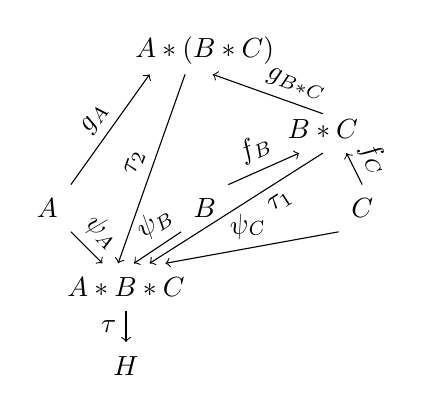
\begin{tikzpicture}
            \node at (0,2) {$A$};
            \node at (2,2) {$B$};
            \node at (4,2) {$C$};
            \node at (2,4) {$A*(B*C)$};
            \node at (3.5,3) {$B*C$};
            \node at (1,1) {$A*B*C$};
            \node at (1,0) {$H$};
            \draw [->] (0.3,2.3)-- node [above, pos=0.5, sloped] {$g_{A}$} (1.3,3.7);
            \draw [->] (1,0.7)-- node [left, pos=0.5] {$\tau$} (1,0.3);
            \draw [->] (2.3,2.3)-- node [above, pos=0.5, sloped] {$f_{B}$} (3.2,2.7);
            \draw [->] (4,2.3)-- node [above, pos=0.5, sloped] {$f_{C}$} (3.8,2.7);
            \draw [->] (3.5,3.2)-- node [above, pos=0.3, sloped] {$g_{B*C}$} (2.1,3.7);
            \draw [->] (0.3, 1.7)-- node [above, pos=0.5, sloped] {$\psi_{A}$} (0.7,1.3);
            \draw [->] (1.7, 1.7)-- node [above, pos=0.3, sloped] {$\psi_{B}$} (1.1,1.3);
            \draw [->] (3.7, 1.7)-- node [above, pos=0.5, sloped] {$\psi_{C}$} (1.5,1.3);
            \draw [->] (1.75,3.7)-- node [above, pos=0.5, sloped] {$\tau_{2}$} (0.9,1.3);
            \draw [->] (3.5,2.7)-- node [below, pos=0.3, sloped] {$\tau_{1}$} (1.3,1.3);
        \end{tikzpicture}
    \end{figure}

    $\psi_{A}:A\to A*B*C$, $\psi_{B}:B\to A*B*C$, $\psi_{C}:C\to A*B*C$. $B*C$ is the coproduct of $B,C$, so there exists unique $\tau_{1}:B*C\to A*B*C$ with $\tau_{1}f_{B}=\psi{B}$, $\tau_{1}f_{C}=\psi{C}$. $A*(B*C)$ is coproduct of $B*C$ and $A$, so there exists unique $\tau_{2}:A*(B*C)\to A*B*C$ with $\tau_{2}g_{A}=\psi{A}$, $\tau_{2}g_{B*C}=\tau_{1}$. For any $H$ with $\varphi_{A}:A\to H$, $\varphi_{B}:B\to H$, $\varphi_{C}:C\to H$. There exists unique $\tau:A*B*C\to H$ with $\varphi_{B}=\tau\psi_{B}=\tau\tau_{2}(g_{B*C}f_{B})$, $\varphi_{C}=\tau\psi_{C}=\tau\tau_{2}(g_{B*C}f_{C})$, $\varphi_{A}=\tau\varphi_{A}=\tau\tau_{2}g_{A}$. $\tau\tau_{2}$ is unique hence $A*(B*C)$ is coproduct of $A$, $B$, $C$. So $A*B*C\cong A*(B*C)$. Similarly $(A*B)*C\cong A*B*C\cong A*(B*C)\Rightarrow (A*B)*C\cong A*(B*C)$.
\end{answer}

$$ $$

\begin{ex}
    If $N$ is normal subgroup of $A*B$ generated by $A$, then $(A*B) /N\cong B$.
\end{ex}

\begin{answer}
    Assume $a_{i_{11}},a_{i_{12}}\cdots\in A$, $b_{j_{11}},b_{j_{12}}\cdots\in B$. Consider homomorphism $\varphi_{B}:A*B\to B$ given by $1\mapsto e$ and \\$(a_{i_{11}}, a_{i_{12}},\dots,a_{i_{1m_{1}}},b_{j_{11}}, \dots, b_{j_{1n_{1}}},a_{i_{21}},\dots)$. It's easy to check $\varphi_{B}$ is well defined. Then $\forall x\in \mathrm{Ker}\varphi_{B}$, no word from $B$ is in $X$, so $\mathrm{Ker}\varphi_{B}\subset\left\langle A\right\rangle$. $\forall a\in\left\langle A\right\rangle$, $\varphi_{B}(a)=1\Rightarrow\left\langle A\right\rangle\subset \mathrm{Ker}\varphi_{B}$. Hence $\mathrm{Ker}\varphi_{B}=\left\langle A\right\rangle$, $(A*B) /N\cong B$.
\end{answer}

$$ $$

\begin{ex}
    If $G$ and $H$ each have more than one element, then $G*H$ is an infinite group with center $\left\langle e\right\rangle$.
\end{ex}

\begin{answer}
    Actually this need $G\neq H$. For any $x\in G*H$, $x\neq e$. WLOG, assume the first word of $x$ belongs to $G$, then take any $h\in H$, $xh\neq hx$. Hence the center must be $\{e\}$. $G*H$ is infinite since $\left\langle ab\right\rangle\subset G*H$ is infinite.
\end{answer}

$$ $$

\begin{ex}
    A free group is a free product of infinite cyclic groups.
\end{ex}

\begin{answer}
    Assume $G$ is the free group on the set $X$. From \textbf{Exercise 1.4.10}, the finite cyclic group is isomorphic to $\mathbf{Z}$. Since the free functor $F:\mathrm{\mathbf{Set}} \to \mathrm{\mathbf{Grp}}$ preserves coproducts. $X=\coprod\limits_{x\in X}\{1\}$, $F(\{1\})=\mathbf{Z}$, we have $G=F(X)=F(\coprod\limits_{x\in X}\{1\})=\coprod\limits_{x\in X}F(\{1\})=\mathop{*}\limits_{x\in X}\mathbf{Z}$.
\end{answer}

$$ $$

\begin{ex}
    If $G$ is the group defined by generators $a, b$ and relations $a^{2}=e$, $b^{3}=e$, then $G\cong Z_{2}*Z_{3}$.
\end{ex}

\begin{answer}
    $Z_{3}\cong \{e,a\}$, $Z_{3}\cong \{e,b,b^{2}\}$. $F(\{a\})*F(\{b,b^{2}\})=F(\{a,b,b^{2}\})=F(\{a,b|a^{2}=b^{3}=e\})=G$. $F(\{a\})=\{e,a\}$, $F(\{b\})=\{e,b,b^{2}\}$. So $G\cong Z_{2}*Z_{3}$.
\end{answer}

$$ $$

\begin{ex}
    If $f:G_{1}\to G_{2}$ and $g:H_{1}\to H_{2}$ are homomorphisms of groups, then there is a unique homomorphism $h:G_{1}*H_{1}\to G_{2}H_{2}$ such that $h|G_{1}=f$ and $h|H_{1}=g$.
\end{ex}

\begin{answer}
    \begin{figure}[H]\centering
        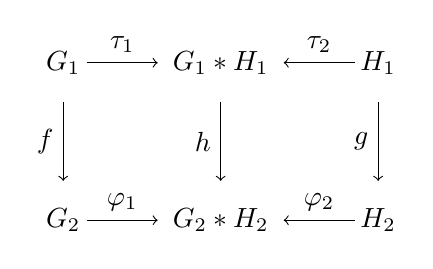
\begin{tikzpicture}
            \node at (0,0) {$G_{2}$};
            \node at (2,0) {$G_{2}*H_{2}$};
            \node at (4,0) {$H_{2}$};
            \node at (0,2) {$G_{1}$};
            \node at (2,2) {$G_{1}*H_{1}$};
            \node at (4,2) {$H_{1}$};
            \draw [->] (0.3,0)-- node [above, pos=0.5] {$\varphi_{1}$} (1.2,0);
            \draw [->] (3.7,0)-- node [above, pos=0.5] {$\varphi_{2}$} (2.8,0);
            \draw [->] (0.3,2)-- node [above, pos=0.5] {$\tau_{1}$} (1.2,2);
            \draw [->] (3.7,2)-- node [above, pos=0.5] {$\tau_{2}$} (2.8,2);
            \draw [<-] (0,0.5)-- node [left, pos=0.5] {$f$} (0,1.5);
            \draw [<-] (2,0.5)-- node [left, pos=0.5] {$h$} (2,1.5);
            \draw [<-] (4,0.5)-- node [left, pos=0.5] {$g$} (4,1.5);
        \end{tikzpicture}
    \end{figure}

    From the property of coproduct. $h$ is a unique homomorphism satisfies $h\tau_{1}=f\varphi_{1}$, $h\tau_{2}=f\varphi_{2}$.
\end{answer}